\section{Introduzione}

\subsection{PadovaCard ora}
PadovaCard è un pacchetto ideato per chi desidera visitare la città di Padova.  Suoi punti di forza sono:
\begin{itemize}
\item Utilizzo gratuito dei mezzi di trasporto pubblici comunali;
\item Parcheggio gratuito in alcune aree;
\item Noleggio di veicoli, biciclette e segway a prezzo scontato;
\item Accesso gratuito alle strutture convenzionate.
\end{itemize}
\`E acquistabile con validità di 48 e 72 ore, contate dal momento in cui viene ritirata allo sportello informazioni assistenza turistica (\glossario{IAT}).
La carta si presenta come in Figura \ref{immaginePadovaCard}, e non possiede nessun tipo di circuito integrato, banda magnetica o codice stampato. 
Proprio per questo motivo, nonostante sia una tessera personale e non cedibile, non c'è modo di verificarne l'intestatario.\\

\begin{figure}[H]
\centering
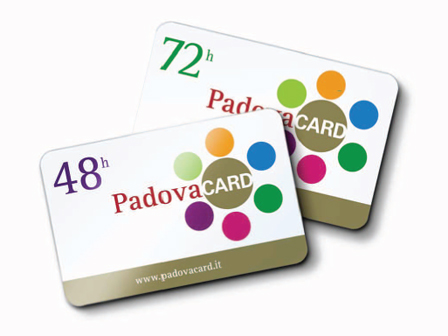
\includegraphics[width=0.6\textwidth]{images/padovacard.jpg}
\caption{Veste grafica dell'attuale PadovaCard}\label{immaginePadovaCard}
\end{figure}

Per acquistare una PadovaCard l'\glossario{utente} può recarsi ad uno degli sportelli IAT che si trovano sul territorio della città di Padova o in uno dei punti vendita autorizzati (hotel, tabaccherie, etc.).\\

\label{cappella}
La \cappella è uno tra i luoghi d'interesse più visitati, ed è convenzionato con PadovaCard. La visita alla \cappella presenta un ingresso contingentato, ovvero il numero di visitatori per ogni visita è fissato, e per questo è necessario prenotare la propria visita, definendo data e fascia oraria. Non è possibile visitare la \cappella senza prenotazione. \\

Tale vincolo fa si che chiunque acquisti una PadovaCard con l'intenzione di visitare la \cappella è obbligato a prenotarne la visita e questo è possibile farlo se si acquista la PadovaCard in un punto vendita autorizzato oppure attraverso la piattaforma \glossario{\vivaticket}.
\`E inoltre attivo un call center che permette agli utenti di acquistare una PadovaCard collegata ad un ingresso in \cappella.
In questi ultimi due casi la PadovaCard verrà poi ritirata presso un punto vendita o direttamente alla \cappella.\\

I principali problemi di funzionamento dell'attuale PadovaCard sono:
\begin{itemize}
\item La PadovaCard non è nominativa;
\item Il sistema non è informatizzato e non prevede alcun tipo di tracciamento o statistica;
\item L'utente è obbligato in tutti i casi a passare da uno IAT per il ritiro della PadovaCard;
\item La piattaforma di vendita è frammentata e non comunica pienamente le offerte della PadovaCard;
\item Il sistema di vendita è frammentato tra OSS e \tlite.
\end{itemize}

La nuova PadovaCard si pone l'obbiettivo di risolvere questi problemi.



\subsection{OSS}\label{oss}
\subsubsection{Overview}
\glossario{OSS} è una piattaforma sviluppata da \net per la gestione del call center, degli sportelli \glossario{IAT} e dei relativi operatori.
Gli operatori si autenticano su questo software per gestire la vendita dell'attuale PadovaCard e di ogni altra merce in vendita agli sportelli \glossario{IAT}. 
OSS permette agli operatori di visualizzare il rendiconto delle vendite e al personale operatvio di compiere interrogazioni sulla base di dati.

\subsubsection{Dettagli tecnici}
Il software è scritto in \glossario{Cake Php} e si basa sull'architettura \glossario{MVC}. Come previsto da MVC sono presenti dei model, uno per ogni tabella del database, tali model si occupano di comunicare col database e di manipolare e verificare i dati che vengono estratti ed inseriti.
Per ogni model è presente un controller, che fornisce la logica al sistema attraverso vari metodi. Ad ogni controller sono collegate più view, ovvero le interfaccie utente. Una view è una pagina con cui l'utente interagisce e ogni view deve essere associata ad un controller di cui chiamerà i metodi.\\

Il web server su cui gira il servizio è \glossario{Apache} e il database su cui si basa il sistema è un database \glossario{MySql}.



\subsection{\tlite}
\tlite è il software sviluppato da \glossario{\charta} che si trova dietro la piattaforma \glossario{\vivaticket}, e che gli operatori utilizzano per gestire la vendita delle PadovaCard\footnote{Sia OSS che \tlite possono vendere la PadovaCard, salvando i dati relativi alla vendita in due diverse basi di dati. Si tratta di un problema dell'attuale sistema.} con annessa prenotazione alla \cappella.
Non trattandosi di un software sviluppato da \net si sono dovuti adattare i requisiti ai limiti imposti da tale software.
Il limite principale è la mancanza di comunicazione tra \tlite e il software sviluppato causato da una mancanza di \glossario{API} pubbliche di \tlite.\\

Si sono comunque rivelate necessarie alcune modifiche minori al software e per questo è stato svolto un incontro tra gli sviluppaotri di \tlite e quelli di \net il cui resoconto è consultabile nell'Appendice \ref{verbale}.
Ai fini di questo documento non è necessario conoscere il funzionamento di \tlite nel suo insieme, mentre i punti d'interesse per la progettazione del nuovo sistema per PadovaCard saranno presentati nella sezione \ref{progettazione}.

\subsection{Lavoro svolto}
Il focus dello stage è stato sui seguenti punti:
\begin{itemize}
\item Analizzare i requisiti del sistema PadovaCard;
\item Progettare un sistema modulare che copra tutti i requisiti obbligatori e permetta di implementare i requisiti facoltativi in modo relativamente semplice;
\item Sviluppare ciò che è stato progettato nei tempi previsti, integrando quanto OSS già offre;
\item Testare il risultato finale assieme agli operatori che andranno ad utilizzare il software, quindi risolvere eventuali difetti trovati o apportare piccole modifiche per facilitare il lavoro degli operatori.
\end{itemize}

\subsubsection{Analisi dei requisiti}
Di seguito viene descritto l'approccio seguito per generare una dettagliata analisi dei requisiti, il cui risultato è presentato nella Sezione \ref{analisideirequisiti}. \\

L'azienda \net ha fornito al tirocinante un documento in cui vengono descritti gli obbiettivi e le criticità del nuovo sistema per la Padovacard. Dallo studio di tale documento il tirocinante ha potuto definire il piano di lavoro dello stage.\\

L'analisi degli obbiettivi e del funzionamento del sistema ad alto livello è stato poi discusso in diverse riunioni tra i membri del team di sviluppo, e i membri di \charta \footnote{Il verbale della riunione è consultabile all'Appendice \ref{verbale}}, ponendo un focus particolare sulle difficoltà inerenti alla \cappella, esposte nella Sezione \ref{cappella}.\\

Da queste riunioni il tirocinante ha estratto i dettagli funzionali dell’applicazione.
Per esprimere in modo chiaro i requisiti individuati si è ricorso al formalismo \glossario{UML} - Casi d'uso, anch'essi visionabili alla Sezione \ref{analisideirequisiti}.\\

L'individuazione dei requisiti è stata fatta corretamente già alla prima iterazione, mentre i casi d'uso e la loro descrizione dettagliata sono stati modificati più volte, al fine di eliminare ogni possibile ambiguità.
\subsubsection{Progettazione}
Questa fase ha avuto inizio con un insieme di requisiti completi. Durante la progettazione ci si è però accorti che alcuni requisiti giudicati implementativamente semplici avrebbero richiesto molte \glossario{ore/uomo} e sono quindi stati declassificati da obbligatori a facoltativi, viceversa alcuni requisiti facoltativi si sono giudicati essenziali per avere un buon sistema e sono quindi stati promossi a obbligatori. Alcuni requisiti sono inoltre stati ulteriorlmente scomposti per permettere una migliore progettazione. \\

Il focus durante la progettazione è stato cercare di riutilizzare il più possibile di quanto OSS già offriva, come interfacce e controller, per questo alcuni controller sono semplicemente stati estesi con nuovi metodi mentre altri sono stati creati ex-novo.\\ 

Molta attenzione è stata posta anche nel progettare in previsione di espansioni future, principalmente per quanto riguarda la base di dati. Il sistema quando completo prevede l'implementazione di tutti i requisiti facoltativi ed è quindi stato importante progettare le componenti in modo tale da evitari grossi costi futuri.\\ 

Per poter dare un idea del software a chi non possiede le necessarie competenze tecniche sono stati realizzati dei mockup dell'interfaccia grafica.

\subsubsection{Sviluppo}
Il problema principale durante la fase di sviluppo è stata la comprensione del codice già esistente e la mancanza di un sistema di versionamento. \\

Il primo problema è stato risolto lavorando a stretto contatto con il creatore della versione originaria di OSS, mentre per risolvere il secondo si è creata una repository \glossario{CVS}. \\

Il codice sorgente è stato documentato con semplici commenti per quanto riguarda il funzionamento nel dettaglio, mentre a livello di classi e metodi si è utilizzato \glossario{PHPDocumentor}, per automatizzare la creazione della documentazione. \\

Il risultato della progettazione è visibile nella Sezione \ref{progettazione}.

\subsubsection{Verifica}
La verifica del software è stata fatta passo passo ad ogni nuova funzionalità implementata. Tale verifica è stata fatta a mano dagli sviluppatori in quanto non sono stati previsti test automatizzati. La verifica finale è stata fatta dagli operatori che andranno poi ad utilizzare il software. \\

Le due verifiche hanno però scopi diversi, quelle effettuate dagli sviluppatori hanno l'obbiettivo di accertarsi che la nuova funzionalità sviluppata non abbia creato bug su quelle precedentemente implementate, mentre quelle effettuate dagli operatori sono state fatte sul software finito e già verificato da parte degli sviluppatori,e il loroobbiettivo è testare sia il software che la validità del manuale, dato che gli operatori si sono basati su quello per capire il funzionamento del software, e testare che durante un vero ciclo di vendita non sorgessero casi non previsiti dal software e che quindi terminavano con un errore. 


\subsection{Risultati a fine stage}
Il periodo di stage è terminato con un software completo e testato, anche se molti dettagli, come ad esempio il contenuto delle email inviate dal sistema non sono stati definiti.
Il software non ha raggiunto l'operatività, principalmente per la mancanza dell'hardware necessario nelle biglietterie delle varie strutture e per la necessità di un periodo di formazione degli operatori. \\

Quando tutti questi vincoli saranno soddisfatti sarà possibile spostare il software dall'ambiente di test a quello definitivo, con l'accortezza di verificare che tutte le impostazione dei due server siano identiche, o in ogni caso che non producano risultati differenti.

